\documentclass[letterpaper,10pt]{article}

%\setlength{\parindent}{0in}
%\usepackage{fullpage} 
\usepackage{amsmath}
\usepackage{amssymb}
\usepackage{enumerate}
\usepackage{graphicx}
\usepackage[table]{xcolor}
\usepackage{dcolumn}
\oddsidemargin 0.0in
\textwidth 6.5in
\newcolumntype{.}{D{.}{.}{-1}}
\newcommand*{\myalign}[2]{\multicolumn{1}{#1}{#2}}

%opening
\title{Homework}
\author{Steve Mazza}
%\date{July 22, 2013}

\begin{document}
\maketitle

\section*{Midterm Project}
\subsection*{Problem 1}
For all of the following, see the attached MATLAB file for the calculation.
\subsubsection*{(a)}
\begin{quote}\begin{description}
	\item[step:] 0.6656
	\item[ramp:] 87.1807
	\item[accel:] 1.1663e+04
\end{description}\end{quote}
\subsubsection*{(b)}
\begin{quote}\begin{description}
	\item[step:] 0.8002
	\item[ramp:] 19.1654
	\item[accel:] 7.0527e+03
\end{description}\end{quote}
\subsubsection*{(c)}
\begin{quote}\begin{description}
	\item[step:] 3.9954
	\item[ramp:] 4.4321e+04
	\item[accel:] 1.9645e+08
\end{description}\end{quote}
\subsubsection*{(d)}
\begin{quote}\begin{description}
	\item[step:] 0.8999
	\item[ramp:] 206.1327
	\item[accel:] 2.1452e+05
\end{description}\end{quote}

\subsection*{Problem 2}
\subsubsection*{(a)}
\subsubsection*{(b)}
\subsubsection*{(c)}
\subsubsection*{(d)}
\subsubsection*{(e)}
\subsubsection*{(f)}
\subsubsection*{(g)}

\section*{Homework 7}
\subsection*{Problem 1}
Root-locus plots of the following functions\dots
\subsubsection*{(a)}
\begin{center}
    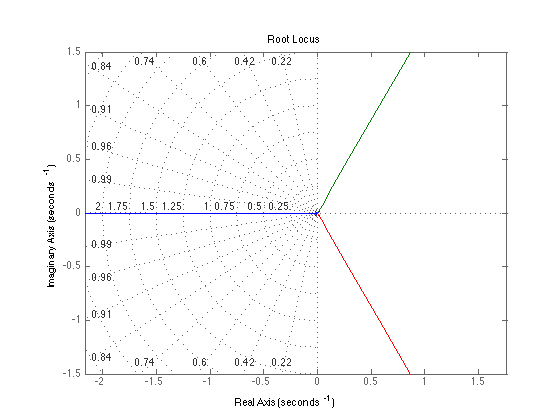
\includegraphics[width=0.6\textwidth]{homework04-7-1-a.png} \\
   $G(s) = \dfrac{1}{(s+0)^{3}}$
\end{center}
\subsubsection*{(b)}
\begin{center}
    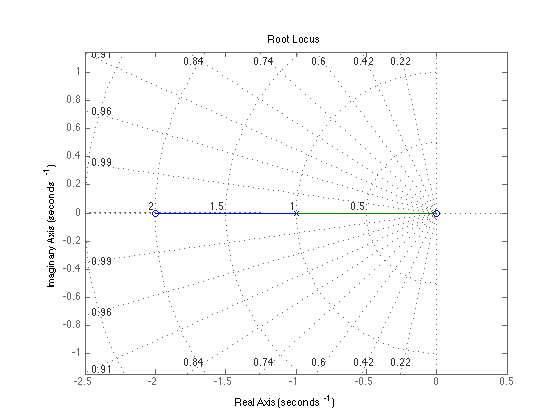
\includegraphics[width=0.6\textwidth]{homework04-7-1-b.png} \\
   $G(s) = \dfrac{(s+0)(s+2)}{(s+1)^{2}}$
\end{center}
\subsubsection*{(c)}
\begin{center}
    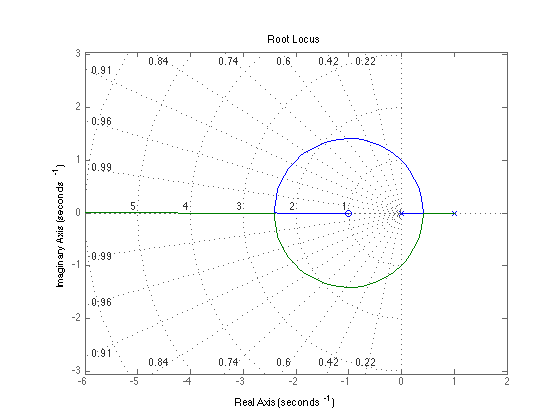
\includegraphics[width=0.6\textwidth]{homework04-7-1-c.png} \\
   $G(s) = \dfrac{s+1}{(s+0)(s-1)}$
\end{center}
\subsubsection*{(d)}
\begin{center}
    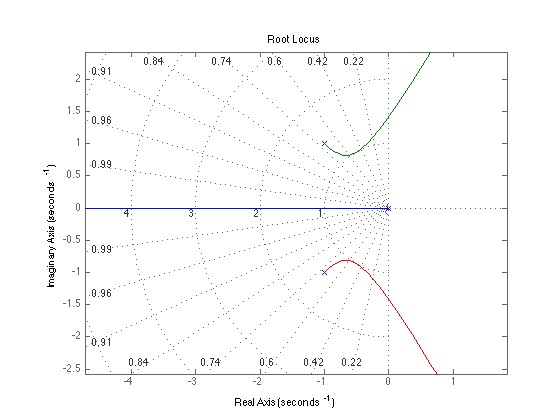
\includegraphics[width=0.6\textwidth]{homework04-7-1-d.png} \\
   $G(s) = \dfrac{1}{(s+0)(s+1+i)(s+1-i)}$
\end{center}
\subsubsection*{(e)}
\begin{center}
    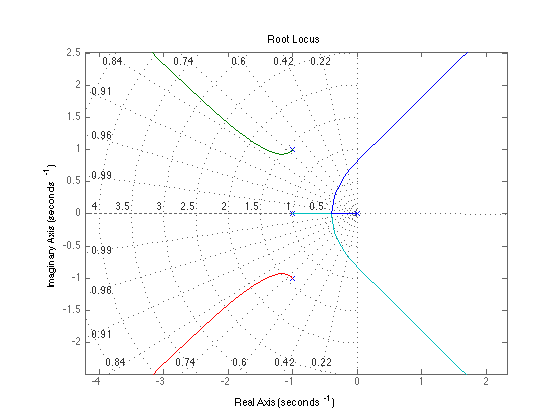
\includegraphics[width=0.6\textwidth]{homework04-7-1-e.png} \\
   $G(s) = \dfrac{1}{(s+0)(s+1+i)(s+1-i)(s+1)}$
\end{center}
\subsubsection*{(f)}
\begin{center}
    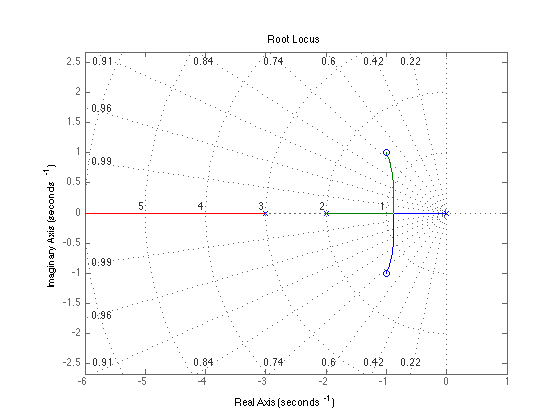
\includegraphics[width=0.6\textwidth]{homework04-7-1-f.png} \\
   $G(s) = \dfrac{(s+1-i)(s+1+i)}{(s+0)(s+2)(s+3)}$
\end{center}
\subsubsection*{(g)}
\begin{center}
    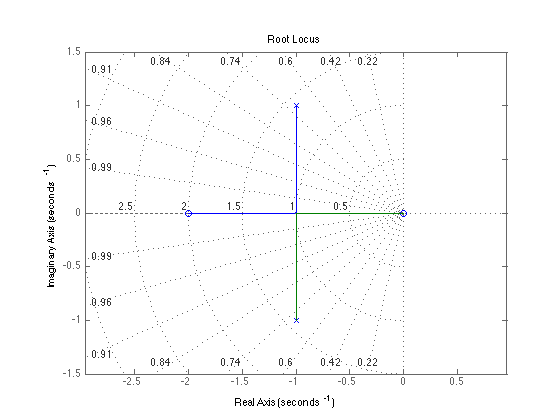
\includegraphics[width=0.6\textwidth]{homework04-7-1-g.png} \\
   $G(s) = \dfrac{(s+0)(s+2)}{(s+1-i)(s+1+i)}$
\end{center}
\subsubsection*{(h)}
\begin{center}
    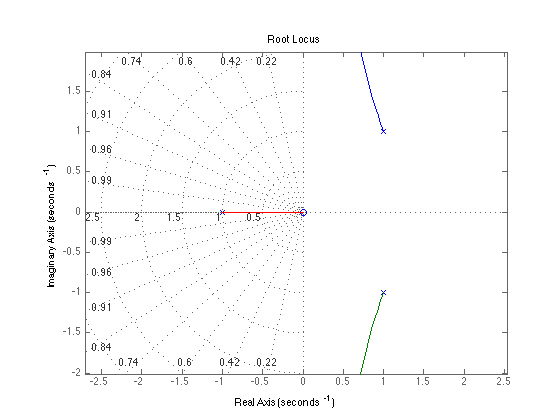
\includegraphics[width=0.6\textwidth]{homework04-7-1-h.png} \\
   $G(s) = \dfrac{(s+0)}{(s+1)(s-1-i)(s-1+i)}$
\end{center}
\subsubsection*{(i)}
\begin{center}
    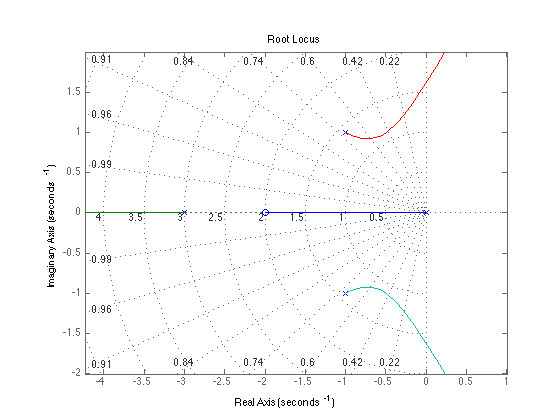
\includegraphics[width=0.6\textwidth]{homework04-7-1-i.png} \\
   $G(s) = \dfrac{(s+2)}{(s+0)(s+3)(s+1-i)(s+1+i)}$
\end{center}

\subsection*{Problem 4}
First we apply our reduction rules to the system an derive the open-loop transfer function as follows:
\begin{align*}
	G(s) &= \dfrac{20}{(s+1)(s+4)} \\
	0 &= \dfrac{\dfrac{20}{(s+1)(s+4)}}{1+\dfrac{20}{(s+1)(s+4)}\times K} \\
	0 &= \dfrac{20}{s^{2}+5s+4+20K} \times \dfrac{1}{s} \\
	0 &= \dfrac{20}{s^{3}+5s^{2}+4s+20Ks} \\
	\dfrac{C(s)}{R(s)} &= \dfrac{20}{s^{3}+5s^{2}+4s+20+20Ks} \\
	&= \dfrac{20}{(s+2i)(s-2i)(s+5)+20Ks} 
\end{align*}
So we have roots at $\pm 2i$ and $-5$.  I then plug the values that I know into the supplied MATLAB script, \texttt{velocity\_feedback.m}, and obtain two values for $k$ satisfying $\zeta = 0.4$: $k = 0.45\times20$ and $k = 1.4\times20$.
\begin{center}
	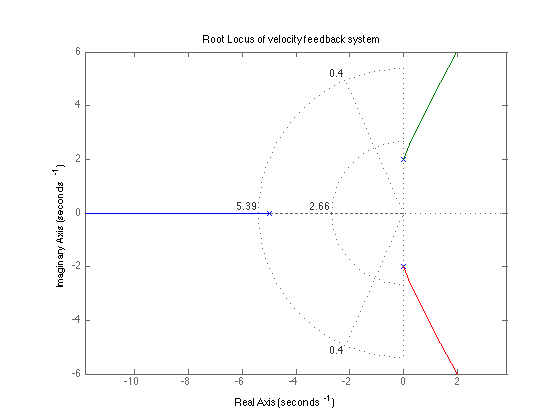
\includegraphics[width=0.49\textwidth]{homework04-7-4a.png}
	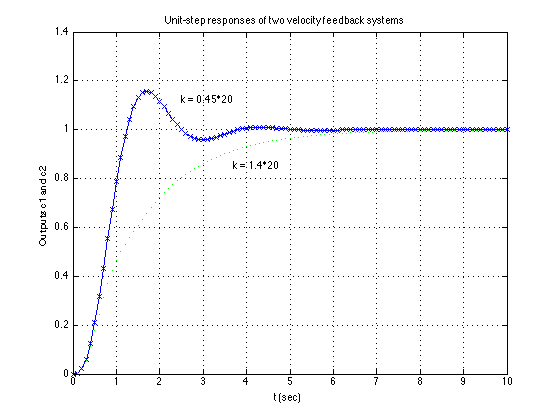
\includegraphics[width=0.49\textwidth]{homework04-7-4b.png}
\end{center}

\subsection*{Problem 5}
Reducing the system, we obtain a transfer function of
$$\dfrac{K_{p}+K_{d}s}{Js^{2}}$$
Removing the unity feedback, we obtain
$$\dfrac{K_{p}+K_{d}s}{Js^{2}+K_{p}+K_{d}s}$$

Determine damping ratio, $\zeta$, for maximum overshoot, $M_{p}$, given:
\begin{align*}
	M_{p} &= e^{-\left(\zeta/\sqrt{1-\zeta^{2}}\right)\pi} \\
	0.1 &= e^{-\left(\zeta/\sqrt{1-\zeta^{2}}\right)\pi} \\
	\zeta &\approx 0.826085
\end{align*}

\end{document}